\documentclass{article}
\usepackage[utf8]{inputenc}
\usepackage[T1]{fontenc}
\usepackage[headheight=12.95494pt,,margin=1in,includefoot]{geometry}
\usepackage{lipsum}
\usepackage{fancyhdr}
\usepackage{setspace}
\usepackage{newunicodechar}
\usepackage{hyperref}
\usepackage{xcolor}
\usepackage{graphicx}
\usepackage{float}
\usepackage{titlesec}
\usepackage{helvet}
\usepackage{tabularx}
\usepackage[page,toc,titletoc,title]{appendix}

\renewcommand{\familydefault}{\sfdefault}
\usepackage[normalem]{ulem}
\titleformat{\section}
  {\large\bfseries\centering}
  {\thesection}{4em}{}
\titleformat{\paragraph}
{\normalfont\normalsize\bfseries}{\theparagraph}{1em}{}
\titlespacing*{\paragraph}
{0pt}{3.25ex plus 1ex minus .2ex}{1.5ex plus .2ex}
\setcounter{secnumdepth}{4}
\newunicodechar{fi}{fi}
\newunicodechar{ff}{ff}
%\usepackage[T1]{fontenc}
\renewcommand{\baselinestretch}{1.7} 
\renewcommand{\headrulewidth}{1pt}
\renewcommand{\footrulewidth}{0pt}
\renewcommand{\contentsname}{table de matière  }
\renewcommand{\listfigurename}{liste des figures  }
\renewcommand{\listtablename}{liste des tableaux}
\setcounter{section}{1}


\pagestyle{fancy}
\fancyhead[R]{rapport de stage}
\begin{document}
\pagenumbering{roman}


\begin{center}
\section*{Dédicaces}

\end{center}
%\addcontentsline{toc}{section}{Dédicaces}

\vspace*{\fill}
\begin{center}
\emph{A mes parents, pour vos sacrifices, vos conseils et vos bénédictions.\\ \vspace{2\baselineskip}
A ma soeur et mon frère, pour le soutien que vous m'avez accordé,\\ \vspace{2\baselineskip}
A mes collègues, pour m'avoir rendu la période de stage agréable,\\ \vspace{2\baselineskip}
A toute ma famille,\\ \vspace{2\baselineskip}
A mes amis et à mes proches,\\ \vspace{2\baselineskip}
A tous ceux qui ont participé à ma formation,\\ \vspace{2\baselineskip}
A tous ceux qui m'ont aidé à réaliser ce travail.\\ \vspace{2\baselineskip}}
\end{center}
\begin{flushright}
\emph{\textbf{Toute ma reconnaissance et ma gratitude...}}
\end{flushright}
\vspace*{\fill} 
\newpage


\begin{center}
\section*{REMERCIEMENTS}\label{sec:remer}
%\addcontentsline{toc}{section}{\numberline{}remerciements}
\end{center}
\vspace*{0.3in}

\textbf{J} ’aimerais exprimer ma gratitude envers Monsieur Aouadi Bacem, mon encadrant au sein du General Assistance connecté. Son soutien, sa collaboration et son assistance m’ont aidée à mieux profiter de mon stage et ses conseils et orientations me furent d’une inestimable utilité.

\textbf{J}e remercie également Monsieur Ben braik Ilyess, un membre de l'équipe, pour son encouragement, ses conseils bien précieux et son encadrement judicieux.


\textbf{M}es remerciements s’adressent également aux membres du jury pour avoir accepté d’évaluer ce travail. J’espère être digne de leur intérêt.

\textbf{F}inalement je remercie tous mes enseignants à l’Ecole Nationale Supérieur d’Ingénieurs de Tunis.
\cleardoublepage
\tableofcontents
\cleardoublepage
\listoffigures
\cleardoublepage
\listoftables
\cleardoublepage
\pagenumbering{arabic}
\setcounter{page}{1}
\pagestyle{fancy}
\fancyhead[L]{}
\begin{center}
\section*{INTRODUCTION GENERALE}
\addcontentsline{toc}{section}{\numberline{}INTRODUCTION GENERALE}
\end{center}
\vspace*{0.3in}
De nos jours, avec la mécanisation de tous les secteurs de l'économie et surtout de la modernisation de plus en plus poussée du trafic routier, nous assistons à une augmentation exponentielle du nombre d'accidents de la route.
\\
Selon les statistiques de l’observatoire national de la sécurité routière, le nombre d'accidents en 2015 a dépassé 7225. La plupart des gens trouvent des difficultés à remplir correctement le constat amiable d'accident. Il y a des autres qui ne disposent pas des sommes nécessaires pour payer les réparations de leur véhicule accidenté et même ne savent pas quel réparateur choisir et donc tombent dans  un long délai d’attente et une mauvaise qualité de réparation. \\
c'est pour cela il faut exploiter l’émergence de technologie informatique pour aider la société à gérer ce flux d'une manière informatisée d’où la nécessité d’une application web dynamique et ergonomique.\\
Dans ce cadre j’ai effectué un stage s'inscrit respectivement dans mon cursus , sur une mission de développement échelonnée sur une période de deux mois entre Juillet et Août 2017.\\
Le directeur Monsieur Aouadi Bacem et sa société "General Assistance connecté"  a d'emblée suscité mon intérêt avec un projet concret lié au développement d’une application web avec une vraie solution innovante et utilisant un nouveau langage, via un Framework simplifiant la création. \\
Dès cette première prise de contact, j'ai su que l'ambiance de travail allait être encourageante et rigoureuse, en intégrant cette structure dynamique et performante.\\
Mes attentes par rapport à mon cursus universitaire étaient notamment de travailler en équipe, de m'adapter à différents environnements matériels et logiciels, mais aussi d'identifier les possibilités et les limites des applications de l'informatique, et enfin d'intégrer les connaissances acquises pour la résolution des problèmes rencontrés.\\
Le projet en soi s'est orienté sur plusieurs axes de travail sur lesquels j'ai dû me focaliser :
\begin{itemize}
\item Planification des sprints(modules).
\item Développement de module administration.
\item développement de module assistance.
\item intégration des modules et déploiment de l'application.
\end{itemize}
Pour ce faire, il a fallu suivre quelques étapes indispensables, préalables au déploiement du projet, en assimilant d'abord les méthodologies de travail, techniques et outils, en s'investissant à participer à de nouvelles fonctionnalités.\\
Dans le premier chapitre, nous présenterons le cadre de notre projet et il présentera aussi notre sprint 0 ou encore la phase de préparation où nous détaillerons les technologies que nous allons manipuler tout au long de notre projet.\\
 Le deuxième chapitre portera sur les étapes de développement.\\
Et notre dernier chapitre sera dédié à la partie de l’intégration des module et comparaison entre les choix utilisé. Nous finirons par une conclusion générale ainsi que la proposition de quelques perspectives. 
\cleardoublepage
\begin{center}
\section*{Chapitre 1 : Etat de l’art}
\addcontentsline{toc}{section}{\numberline{}Chapitre 1 : Etat de l’art}
\end{center}
\subsection{Introduction}
Le présent chapitre est consacré en un premier lieu à la présentation de l’entreprise d’accueil dans laquelle nous avons effectué notre projet de fin d’étude.\\ En deuxième lieu, nous effectuons une étude de l’existant et nous dégageons les défaillances. En troisième lieu, nous présentons notre solution dont le but de remédier à ses limites. En quatrième lieu nous dégageons les besoins fonctionnels et non fonctionnels ainsi que le backlog de produit suivi par la planification des releases et nous terminons par une présentation des technologies et des outils de développement.
\subsection{Présentation de l’organisme d’accueil: Général Assistance Connecté}
Notre stage se déroule au sein de la société Général Assistance Connecté.
Dans la section qui suit, nous allons donner une description légère de l’entreprise, ses missions ainsi que ses secteurs d’activités.  
\subsubsection{Présentation du Général Assistance Connecté }
Général Assistance Connecté est une entreprise d’ingénierie et de services informatique tunisienne. Elle s’est installée à Tunis depuis 2015 et elle compte actuellement moins de 20 employés.\\ Elle est la filiale informatique du groupe Générale Assistance, forte d'un double positionnement d'éditeur de logiciels informatiques, et également de prestataires de service aussi bien dans l'ingénierie logicielle que dans l'administration Système \& réseaux.

\begin{figure}[H]
\centering

\includegraphics[height=1.75in]{gacLogo.png}
\caption[Figure1 : Logo de la société]{Logo de la société}
\label{fig:pic1}
\end{figure}
\subsubsection{Les missions de Général Assistance Connecté }
Les missions du Général Assistance Connecté sont : 
\begin{itemize}
\item Mise à disposition de ressources informatiques compétentes sur les nouvelles technologies,
\item Installation, administration et sécurisation du système et réseau informatique,
\item Développement web et mobile spécifiques aux besoins métiers du client,
\item Développement Back-End, Front-End, Full Stack en utilisant les langages et technologies de pointe.
\end{itemize}
Le secteur d'activité est :

\begin{itemize}
\item Assurance
\end{itemize}

\subsection{Description du contexte du projet}
\subsubsection{Etude de système existant}
L’étude de l’existant est une phase importante pour bien comprendre l'application web et dégager ces fonctionnalités et ces différents points faibles, ce site est consacré pour le groupe Générale Assistance. Il faut signaler que Générale Assistance joue un véritable rôle culturel en participant au développement des services d’assistance aux personnes par la conception de nouvelles prestations répondants aux besoins évolutifs des clients.\\
Aussi,le groupe exploite les nouvelles technologies d’information et de communication pour améliorer les procédures de gestion des sinistres automobile, habitation et santé en maîtrisant leurs coûts.. Le présent site web assure et simplifie les services précédemment cité d’une manière informatisé.
\subsubsection{Critique de l’existant}
Vu le grand nombre de demande d'assurance et de collaborateur, le projet doit être un site de qualité (efficace, fiable, compatible, séduisant…) et permet de satisfaire les cibles pour lesquelles le site est conçu, mais dans notre cas, la Template utilisée par le site n’est pas ergonomique et parfois les informations ne sont pas bien lisibles ainsi que le chargement de quelque page prendre un temps cela à cause de l'emploi excessif d'images ou d'animations et l’absence d’un menu fixe qui permette d'atteindre les pages principales du site quel que soit la page chargée.
\subsubsection{Problématique}
Le client de la société veut satisfaire les cibles pour lesquelles le site est conçu et s’adapter aux utilisateurs en améliorant les services offertes mais le problème c’est que le taux de traitement est important et la méthode utilisé est lente et n'est pas performante, d’où le besoin de migrer le site en intégrant un nouveau design et corrigeant les bugs, de développer les modules complémentaires pour améliorer les services.
\subsubsection{Présentation de la solution proposée}
Dans un souci de migrer le site web de notre client vers une nouvelle version plus ergonomique et ne présentant pas de bug,  notre solution proposée se résume ainsi dans les fonctionnalités suivantes :
\begin{itemize}
\item Migration de site web
\item Développement des modules complémentaires
\end{itemize}

\subsection{Langage et Méthodologie de la conception}
La méthodologie est une démarche organisée rationnellement pour aboutir à un résultat.
Parmi les différentes méthodologies existantes, nous pouvons citer le modèle en cascade utilisé souvent dans les projets simples dont les besoins sont clairs et bien définis dès le début, le modèle en y utilisé pour le développement des applications mobiles, ainsi que le processus unifié et les méthodologies agiles (Scrum \& extrême programming) caractérisées par leurs souplesses et utilisées dans des grands projets.
Pour bien conduire notre projet et nous assurer du bon déroulement des différentes phases, nous avons opté Scrum comme une méthodologie de conception et de développement.\\
Après le choix de la méthodologie, nous avons besoins, d’un langage de modélisation unifiée pour la modélisation de notre projet. Pour concevoir notre système, nous avons choisi UML\footnote{Unified Modeling Language}  comme un langage de modélisation.
Notre choix s'est basé sur les points forts de ce langage notamment sa standardisation et les divers diagrammes qu’il propose. Aussi UML présente le meilleur outil pour schématiser des systèmes complexes sous un format graphique et textuel simplifié et normalisé.
En effet, UML n'est ni un processus ni une démarche, d'où il fallait choisir une méthodologie de conception et de développement que nous devons l'adopter. Voir \hyperref[sec:hello]{Annexe}

\subsubsection{Pilotage du projet avec Scrum}
\paragraph{Planification d’un projet par Scrum}
\uline{Planification du sprint} : Elle s’appuie sur la planification de la « release » réalisée en pente. La première réunion du sprint ne se limite pas à planifier, on y trouve les activités suivantes :
\begin{enumerate}
\item Valider les \guillemotleft stories\guillemotright du Backlog pris en compte dans le sprint, concevoir les solutions.
\item Identifier et estimer les tâches.
\item Prise des tâches par chacun des membres de l’équipe …
\end{enumerate}
\uline{Revue du sprint} : Elle permet de montrer les résultats du développement effectués au cours du sprint, seule une version opérationnelle est montrée.\\
\uline{Rétrospective} : Elle est faite en interne en équipe (avec la présence du Scrum Master), l’objectif est de comprendre ce qui n’a pas bien fonctionné dans le sprint, les erreurs commises et de prendre des décisions pour procéder aux améliorations.\\
\uline{Scrum quotidien} : il s’agit d’une réunion de synchronisation de l’équipe de développement qui se fait debout en 15 minutes maximum au cours de laquelle chacun répond principalement à 3 questions :
\begin{enumerate}
\item Qu’est-ce que j’ai fait hier ?
\item Qu’est-ce que je ferai aujourd’hui ?
\item Quels obstacles me retardent ?
\end{enumerate}
Voir \hyperref[sec:hello1]{Annexe} 
\subsection{Planification et architecture du projet}
\subsubsection{Capture des besoins}
Nous procéderons par l’identification des acteurs puis la description des histoires utilisateurs du futur système
\paragraph{Identification des acteurs}
Nous avons identifié trois acteurs principaux de notre projet à savoir :
\begin{enumerate}
\item[$\bullet$] Le super-administrateur
\item[$\bullet$] L'administrateur( Utilisateur normal,employé dans la societé)
\end{enumerate}
\begin{table}[H]
\centering
\label{tab:tab1} 
 \begin{tabularx}{\textwidth}{|X|X|X|}
\hline
\bfseries{ Acteur} &\bfseries{ Définition} &\bfseries{ Rôle} \\ \hline
Le super-administrateur& Il s’agit de la personne qui possède toute les permissions sur le système. &Il est responsable de la gestion interne des profils.\\
\hline
L'utilisateur normal & Il s'agit de la personne qui possède des permissions bien spécifiques & Il peut utiliser toutes les fonctionnalités de l'application sauf l'ajout d'un autre administrateur et la consultation de l'historique de connexion.\\
\hline
\end{tabularx}
\caption[tableau1 : les acteurs principaux]{les acteurs principaux}
\end{table}
\subsubsection{Les besoins fonctionnels}
\guillemotleft Les besoins fonctionnels expriment une action que doit effectuer le système en réponse à une demande (sorties qui sont produites pour un ensemble donné d’entrées \guillemotright. [3] \\
Dans ce qui suit, nous décrivons les besoins fonctionnels de notre projet appelés dans Scrum : \\ \guillemotleft User stories \guillemotright.
\begin{enumerate}
\item [$\bullet$] \textbf{Le projet permet au super-admin de :} 
	\begin{enumerate}
	 \item [$\ast$] \uline{S’authentifier :}
	 	\begin{enumerate}
     		\item [\textendash]Se connecter à travers un login et un mot de passe en tant que super-admin.\\
			\item [\textendash]Il y a contrôl de saisie de login et mot de passe,session expirée aprés une durée bien déterminée autre que bloquage de compte après trois tentatives erronées.
		\end{enumerate}
	\item [$\ast$] \uline{Changer ces informations personnelles :}
		\begin{enumerate}
     		\item [\textendash]Changer ses informations personnelles à savoir nom, prénom, mot de passe…etc en cas de besoin.
		\end{enumerate}
	\item [$\ast$] \uline{Gestion des rôles :}
		\begin{enumerate}
     		\item [\textendash]Affecter des modifications sur les rôles en ajoutant un nouveau en cas des besoins ou bien en modifiant les profils.
		\end{enumerate}    
	\item [$\ast$] \uline{Gestion des utilisateurs :}
		\begin{enumerate}
     		\item [\textendash] Ajouter,supprimer ou bien modifier le compte d'un utilisateur en remplissant un formulaire. 
		\end{enumerate}	
	\item [$\ast$] \uline{Gestion des contrats :}
		\begin{enumerate}
     		\item [\textendash] Ajouter,supprimer,bloquer,débloquer ou bien modifier un contrat en remplissant un formulaire. 
		\end{enumerate}
	\item [$\ast$] \uline{Gestion des assurés :}
		\begin{enumerate}
     		\item [\textendash] Ajouter,supprimer ou bien modifier le profil d'un assuré en remplissant un formulaire. 
		\end{enumerate}
	\item [$\ast$] \uline{Gestion des marques de voitures :}
		\begin{enumerate}
     		\item [\textendash] Ajouter ou bien modifier les marques des voitures en remplissant un formulaire. 
		\end{enumerate}
	\item [$\ast$] \uline{Gestion des types de services :}
		\begin{enumerate}
     		\item [\textendash] Ajouter,supprimer ou bien modifier un type de service en remplissant un formulaire. 
		\end{enumerate}
	\item [$\ast$] \uline{Gestion des remorqueurs :}
		\begin{enumerate}
     		\item [\textendash] Ajouter,supprimer,bloquer,débloquer ou bien modifier un remorqueur en remplissant un formulaire. 
		\end{enumerate}
	\item [$\ast$] \uline{Gestion des packs :}
		\begin{enumerate}
     		\item [\textendash] Ajouter,supprimer,bloquer,débloquer ou bien modifier un pack en remplissant un formulaire.
 Un pack contient un nombre maximum de kilométrage et de service.Un contrat peut avoir un ou plusieurs packs. 
		\end{enumerate}
	\end{enumerate}
\item [$\bullet$] \textbf{Le projet permet à l'utilisateur normal de :} 
	\begin{enumerate}
	 	\item [$\ast$] Faire toutes les fonctionnalitées offertes au super-admin sauf la gestion des profiles. 
	\end{enumerate}	

\end{enumerate}
\subsubsection{Les besoins non fonctionnels}
\guillemotleft Il s’agit des besoins qui caractérisent le système. Ce sont des besoins en matière de performance, de type de matériel ou le type de conception. Ces besoins peuvent concerner les contraintes d’implémentation (langage de programmation, type SGBD.) \guillemotright.[4]\\
Les besoins non fonctionnels de notre système, appelés dans Scrum «Technical Stories», se décrivent comme suit :
\begin{enumerate}
\item [$\bullet$] \textbf{Contraintes ergonomiques}
	\begin{enumerate}
     		\item [\textendash] La navigation entre les interfaces de notre future site web doit être légère et fluide.
     		\item [\textendash] Les interfaces de notre future application doivent être simples et homogènes.
     		\item [\textendash] L’utilisateur doit être guidé lors de la saisie de certaines informations, afin de respecter les formats des champs de notre base de données.
     \end{enumerate} 
\item [$\bullet$] \textbf{Contraintes techniques} 
	\begin{enumerate}
     		\item [\textendash] Les mots de passe doivent être cryptés au niveau de la base de données afin de garder sécurisé l’accès à l’espace administration.
     		\item [\textendash] Les requêtes doivent être optimisées afin d’assurer un temps de réponse minimal.
     		
     \end{enumerate}  
\end{enumerate}
\subsubsection{Backlog de produit}
Le Backlog produit est utilisé pour planifier la release et aussi à chaque sprint, lors de la réunion de planification du sprint pour décider du sous-ensemble qui sera réalisé. Ses éléments sont classés par ordre de priorité ce qui permet de définir l’ordre de réalisation.
Pour chaque user story on identifie le rang, l’estimation, l'importance et la description.\\
Voir \hyperref[sec:hello2]{Annexe}.\\
Le tableau suivant décrit le product backlog de notre projet.
\begin{table}[H]
\centering
\label{tab:tab2} 
 \begin{tabularx}{\textwidth}{|X|X|X|X|}
\hline
\bfseries{ Id} &\bfseries{ Nom} &\bfseries{ Description} &\bfseries{ Priorité} \\ \hline
1& Développement de module administration &Le super admin peut bénéficier de fonctionnalités d'administration de l'application & 5\\
\hline
2& Développement de module d'assistance &Préparer l'environnement de travail pour tous les utilisateurs de l'application & 8\\
\hline 
3&Intégration des modules d'administration et d'assistances &Fournir une application complète prête à utiliser & 13\\
\hline
\end{tabularx}
\caption[tableau2 : Backlog de produit]{Backlog de produit}
\end{table}
\subsubsection{Planification de release}
La réunion de planification des sprints est une étape importante dans SCRUM. Le planning de travail et l'identification du Backlog des sprints sont les buts de cette réunion. Durant ce meeting, la durée de chaque sprint est décidée selon la complexité du contexte et la taille de l'équipe.\\
La planification de Sprint répond aux questions suivantes :
\begin{enumerate}
\item Qu’est-ce qui peut être terminé au cours de ce Sprint ?
\item Comment sera effectué le travail choisi ?
\end{enumerate}
Et donc, une succession de Releases est le produit de cette réunion pour organiser le travail de l'équipe. Un Release est une série de Sprints qui se termine quand les incréments successifs constituent un produit présentant suffisamment de valeurs à ses utilisateurs. Dans notre cas, nous avons décidé de découper notre projet en trois Releases.
\begin{figure}[H]
\centering
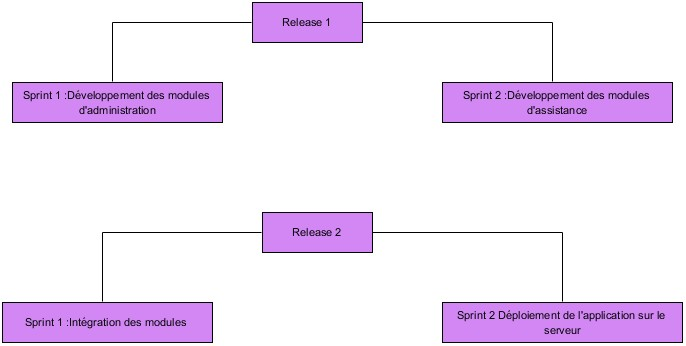
\includegraphics[height=2.8in]{Planification.jpg}
\caption[Figure 2 : Planification de release]{Planification de release}
\label{fig:pic2}
\end{figure}
\subsubsection{Identification de l’équipe scrum}
\begin{table}[H]
\centering
\label{tab:tab3} 
 \begin{tabularx}{\textwidth}{|X|X|}
\hline
\bfseries{ Rôles Scrum} &\bfseries{ Personnes affectés} \\ \hline
Product Owner& Toukebri Mohamed Arbi \\
\hline
Scrum Master& Aouadi Bacem \\
\hline 
Team&Choubani amir, Dahmeni Senda, Ardhaoui Aymen, Turki nessrine.\\
 
\hline
\end{tabularx}
\caption[tableau3 : Identification de l'équipe scrum]{Identification de l'équipe scrum}
\end{table}
\subsubsection{Diagramme de cas d’utilisation initiale}
Maintenant, nous allons présenter les différents besoins fonctionnels de notre système exprimés précédemment d'une manière informelle en utilisant le digramme de cas d'utilisation d'UML.\\
La figure \ref{fig:pic3} illustre le diagramme de cas d'utilisation global de notre système.

\begin{figure}[H]
\centering
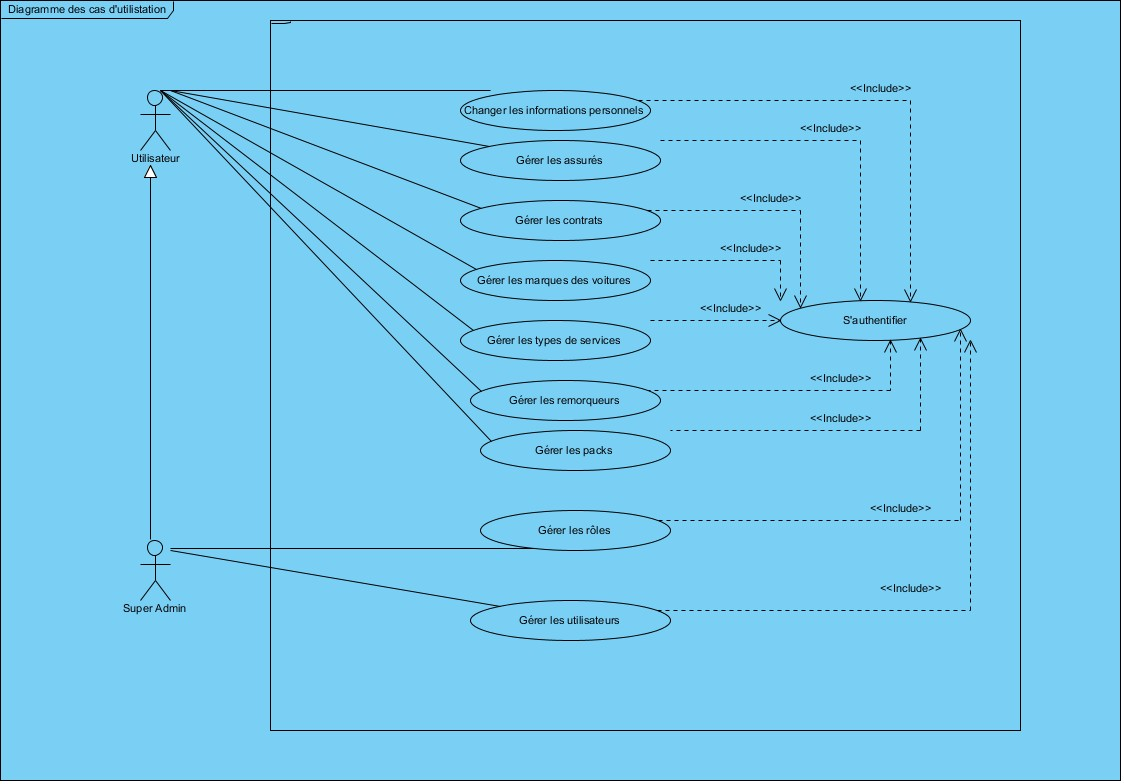
\includegraphics[height=5.6in]{UseCaseDiagram1.jpg}
\caption[Figure3 : Diagramme de cas d'utilisation]{Diagramme de cas d'utilisation}
\label{fig:pic3}
\end{figure}
\cleardoublepage
\subsubsection{Technologie et outils de développement}
Dans cette partie, nous décrivons tous les outils matériels et logiciels de développement et de conception, avec lesquels on a réalisé ce projet. Nous allons commencer par une brève description des environnements Spring Boot et Angular, de l’architecture de notre application, et nous allons finir par les outils de développement utilisé pour réaliser ce projet.
\paragraph{Présentation des environnements de travail}
\begin{enumerate}
\item [$\bullet$] \textbf{Spring Boot}
\begin{figure}[H]
\centering

\includegraphics[height=1.5in]{springboot.png}
\caption[Figure4 : Logo de Spring Boot ]{Logo de Spring Boot [5]}
\label{fig:pic4}
\end{figure}
Spring Boot est un nouveau framework créé par l'équipe de chez Pivotal, conçu pour simplifier le démarrage et le développement de nouvelles applications Spring.\\
Voir \hyperref[sec:hello3]{Annexe}
\item [$\bullet$] \textbf{Angular}
\begin{figure}[H]
\centering

\includegraphics[height=1.5in]{angular-2-logo.jpg}
\caption[Figure5 : Logo de Angular  ]{Logo de Angular [6]}
\label{fig:pic5}
\end{figure}
Angular est un framework Javascript pour créer des applications monopages,web et mobile.\\
Il supporte plusieurs langage : ES5,ES6 et typescript.C'est une version qui suit AngularJS et qui a introduit un travail complètement différent en utilisant l'orienté objet (notion de composant).
\item [$\bullet$] \textbf{PostgreSQL}
Pour la gestion de base de donnée , on a utilisé PostgreSQL qui est similaire à MYSQL.
\end{enumerate}
\paragraph{Architecture utilisée}
L’architecture en couches de notre système se base sur le patron (modèle) de conception MVC (Model View Controller).
\begin{figure}[H]
\centering
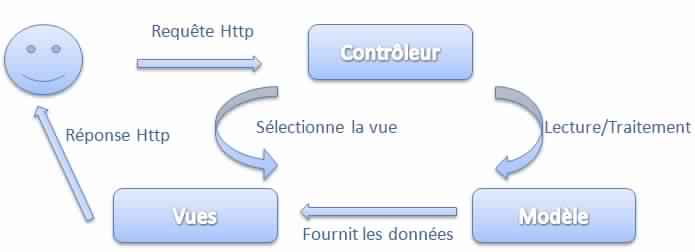
\includegraphics[height=2.6in]{MVC.jpg}
\caption[Figure7 : modèle MVC  ]{modèle MVC [7]}
\label{fig:pic7}
\end{figure}
Modèle-Vue-Contrôleur est un motif d'architecture logicielle destiné pour les applications web. Le motif est composé de trois types de modules ayant trois responsabilités différentes : les modèles, les vues et les contrôleurs.\\
Voir \hyperref[sec:hello4]{Annexe}
\subsubsection{Environnement technique de travail}
Le tableau détaille la configuration matérielle de machine de développement et de déploiement utilisée ainsi que les différents logiciels qui y sont installés :

\begin{table}[H]
\centering
\label{tab:tab4} 
 \begin{tabularx}{\textwidth}{|X|X|}
\hline
 Machines & Asus \\ \hline
Propriétaire& Général Assistance Connecté \\
\hline
Processeur & I7\\
\hline
RAM & 8 GO \\
\hline
Système d’exploitation & UBUNTO 16.04 \\
\hline
\end{tabularx}
\caption[tableau4 : Environnement matérielle]{Environnement matérielle}
\end{table}
\paragraph{Outil de conception}
Visual Paradigm for Unified Modeling Language (VP-UML) est un outil UML. L'outil est conçu pour un large éventail d'utilisateurs, y compris les ingénieurs logiciels, analystes système, analystes et architectes système, ou pour quiconque est intéressé par la construction de manière fiable des systèmes de logiciels à grande échelle en utilisant une approche orientée objet.
\paragraph{Outils de développement}
Dans cette partie nous allons décrire les outils de développement utilisé pour réaliser ce projet.

\begin{center}

\includegraphics[height=0.2in]{npm.png}\\

\includegraphics[height=0.2in]{gitLab.png}\\

\includegraphics[height=0.4in]{VSCode.png}\\

\includegraphics[height=0.4in]{pgAdmin.jpg}\\
\vspace{0.5cm}

\includegraphics[height=0.4in]{eclipse.jpg}
\end{center}
\cleardoublepage

\paragraph{Langages de programmation}
\begin{enumerate}
\item [$\bullet$] \textbf{ Java Entreprise Edition}
\item[$\bullet$] \textbf{ TypeScript}
\item[$\bullet$] \textbf{ Bootstrap 4}
\item[$\bullet$] \textbf{ HTML 5}
\item [$\bullet$] \textbf{ CSS 3} 
\item[$\bullet$] \textbf{ SCSS}
\end{enumerate}
voir annexe.
\subsection{Conclusion}
Dans ce chapitre nous avons présenté le cadre général de notre projet en déterminant la problématique et en proposant la solution envisagée pour faire face à la situation courante. Nous avons dévoilé le langage et la méthodologie de conception qui seront utilisés dans les prochains chapitres de ce rapport. Nous avons présenté le Sprint 0 qui, est en fait une phase de préparation pendant laquelle on a construit notre backlog du produit en se basant sur les besoins fonctionnels et non fonctionnels.\\ En plus, nous avons découpé notre projet en des releases qui formeront les chapitres suivants. Et finalement, nous avons défini les technologies et les environnements de développement ainsi que l’architecture globale de l’application.
Dans le chapitre suivant nous abordons le release 1 dans laquelle nous allons décrire les sprints à réaliser.
\cleardoublepage
\setcounter{section}{2}

\section*{Chapitre 2 :  Release 1 " Développement des modules "}
\addcontentsline{toc}{section}{\numberline{} Chapitre 2 : Release 1 " Développement des modules "}
\setcounter{subsection}{0}
\subsection{Introduction}
Après avoir entamé le release 0 de projet , nous
pouvons maintenant passer au premier release \guillemotleft Gestion d'administration et d'assistance \guillemotright . En effet, ce
release constitue un objectif principal de notre projet puisqu'il permet de gérer l'accés à
l'application et contient les tâches principales .
\subsection{Sprint 1 : Module d'administration}
Au niveau de ce sprint, nous commençons par présenter le diagramme des classes nécéssaires à l'implémentation. Ensuite, on présentera
la conception avec les diagrammes de cas d'utilisation et de  séquences. 
\begin{enumerate}
\item[$\bullet$] \textbf{ Diagramme des classes}
\begin{figure}[H]
\centering
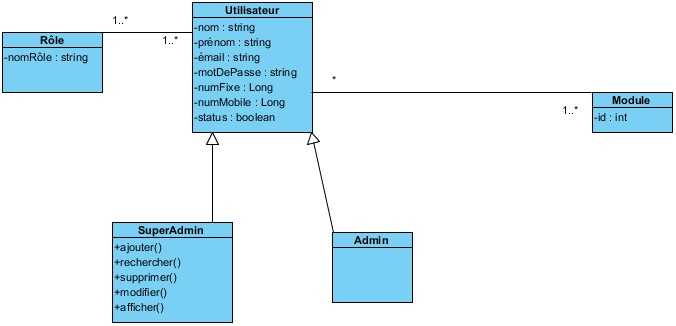
\includegraphics[height=3in]{DiagClass1.jpg}
\caption[Figure9 : Diagramme de classe de module administration]{Diagramme de classe de module administration}
\label{fig:pic9}
\end{figure}
\item[$\bullet$] \textbf{ Diagramme de cas d'utilisation}\\

\begin{figure}[H]
\centering
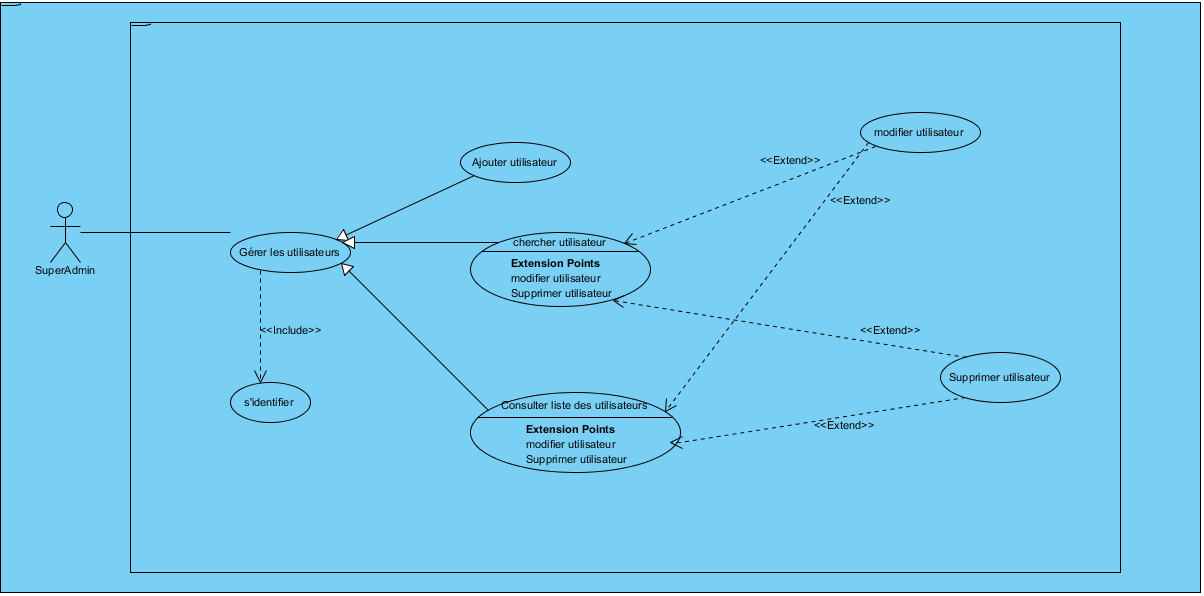
\includegraphics[height=3.7in]{UseCaseDiagram2.png}
\caption[Figure10 : Diagramme de cas d'utilisation " gérer utilisateur "]{Diagramme de cas d'utilisation " gérer utilisateur "}
\label{fig:pic10}
\end{figure}
Le diagramme de cas d'utilisation présenté par la figure \ref{fig:pic10} décrit la gestion des
utilisateurs du système par l'administrateur. Ce diagramme nous montre que l'administrateur ne peut faire sa gestion qu'après identification.Ainsi que la modification ou la
suppression d'un utilisateur ne peut être effectuer qu'après consultation des utilisateurs
ou recherche de ce dernier .
\end{enumerate}
\subsubsection{Description textuelle du cas d'utilisation "ajouter un utilisateur"}

Nous allons réaliser une description textuelle du scénario de ajout d'un utilisateur
pour mieux connaître les étapes à suivre pour que l'administrateur réussit cette ajout.\\
Cette description est présentée par le tableau \ref{tab:tab5}.
\begin{table}[H]
\centering
 \begin{tabularx}{\textwidth}{|X|X|}
\hline
 \textbf{Titre} & \textbf{Ajouter un utilisateur} \\ \hline
\textbf{Résumé} & Ajouter un utilisateur de l'application à la base de données \\
\hline
\textbf{Acteurs} & Super Administrateur\\
\hline
\textbf{Précondition} & S'identifier \\
\hline
\textbf{Postcondition} & Un nouvel utilisateur est sauvegardé \\
\hline
\textbf{Scénario nominal} & \begin{enumerate}
\item l'administrateur saisi les données du nouvel utilisateur
\item l'administrateur appui sur le bouton sauvegarder pour
valider l'ajout
\item l'application affiche un message de succès.
\end{enumerate} \\
\hline
\textbf{Scénario alternatif} & \begin{enumerate}
\item L'administrateur effectue une erreur de saisi(formulaire non entièrement rempli . . .)
\item L'application affche un message d'erreur
\item le scénario nominal reprend au point 1.
\end{enumerate} \\
\hline
\end{tabularx}
\caption[tableau 5 : Tableau descriptif du cas d'utilisation "ajouter un utilisateur"]{Tableau descriptif du cas d'utilisation "ajouter un utilisateur"}
\label{tab:tab5}
\end{table}
\subsubsection{Description textuelle du cas d'utilisation "chercher un utilisateur"}
Nous allons réaliser un tableau descriptif \ref{tab:tab6} du scénario de la recherche d'un utilisateur
pour mieux connaître les étapes à suivre pour que l'administrateur réussit cette
tâche.
\begin{table}[H]
\centering
 \begin{tabularx}{\textwidth}{|X||X|}
\hline
 \textbf{Titre} & \textbf{Chercher un utilisateur} \\ \hline
\textbf{Résumé} & Chercher un utilisateur \\
\hline
\textbf{Acteurs} &Super Administrateur\\
\hline
\textbf{Précondition} & S'identifier \\
\hline
\textbf{Postcondition} & La liste des utilisateurs est affichée. \\
\hline
\textbf{Scénario nominal} & \begin{enumerate}
\item l'administrateur saisi le nom et prénom de l'utilisateur
\item l'application affiche une liste des utilisateurs qui porte
le même nom
\end{enumerate} \\
\hline
\textbf{Scénario alternatif} & \begin{enumerate}
\item L'administrateur saisi des données erronées
\item le scénario nominal reprend au point 1.
\end{enumerate} \\
\hline
\end{tabularx}
\caption[tableau 6 : Tableau descriptif du cas d'utilisation "chercher un utilisateur"]{Tableau descriptif du cas d'utilisation "chercher un utilisateur"}
\label{tab:tab6}
\end{table}
\subsubsection{Description textuelle du cas d'utilisation "consulter liste des utilisateurs"}
Nous allons réaliser une description textuelle du scénario de la consultation de la
liste des utilisateurs pour mieux connaître les étapes à suivre pour que l'administrateur
réussit cette consultation.
Cette description est présentée par le tableau \ref{tab:tab7}
\begin{table}[H]
\centering
 \begin{tabularx}{\textwidth}{|X||X|}
\hline
 \textbf{Titre} & \textbf{Consulter la liste des utilisateurs} \\ \hline
\textbf{Résumé} & Consulter la liste des utilisateurs \\
\hline
\textbf{Acteurs} &Super Administrateur\\
\hline
\textbf{Précondition} & S'identifier \\
\hline
\textbf{Postcondition} & La liste des utilisateurs est affichée. \\
\hline
\textbf{Scénario nominal} & \begin{enumerate}
\item l'administrateur appui sur la page de navigation
voulu \guillemotleft liste les utilisateurs \guillemotright
\item l'administrateur consulte la liste des utilisateurs.
\end{enumerate} \\
\hline
\textbf{Scénario alternatif} & \begin{enumerate}
\item L'administrateur sélectionne la page de
navigation non voulu
\item le scénario nominal reprend au point 1.
\end{enumerate} \\
\hline
\end{tabularx}
\caption[tableau 7 : Tableau descriptif du cas d'utilisation "consulter liste des utilisateurs"]{Tableau descriptif du cas d'utilisation "consulter liste des utilisateurs"}
\label{tab:tab7}
\end{table}
\subsubsection{Conception}
Après la spécification des différentes fonctionnalités du backlog de ce sprint, nous
passons à la phase de conception pour mieux expliquer ses fonctionnalités à l'aide des
diagrammes de séquence.
\subsubsection{Diagramme de séquence "Ajouter un utilisateur"}
\begin{figure}[H]
\centering
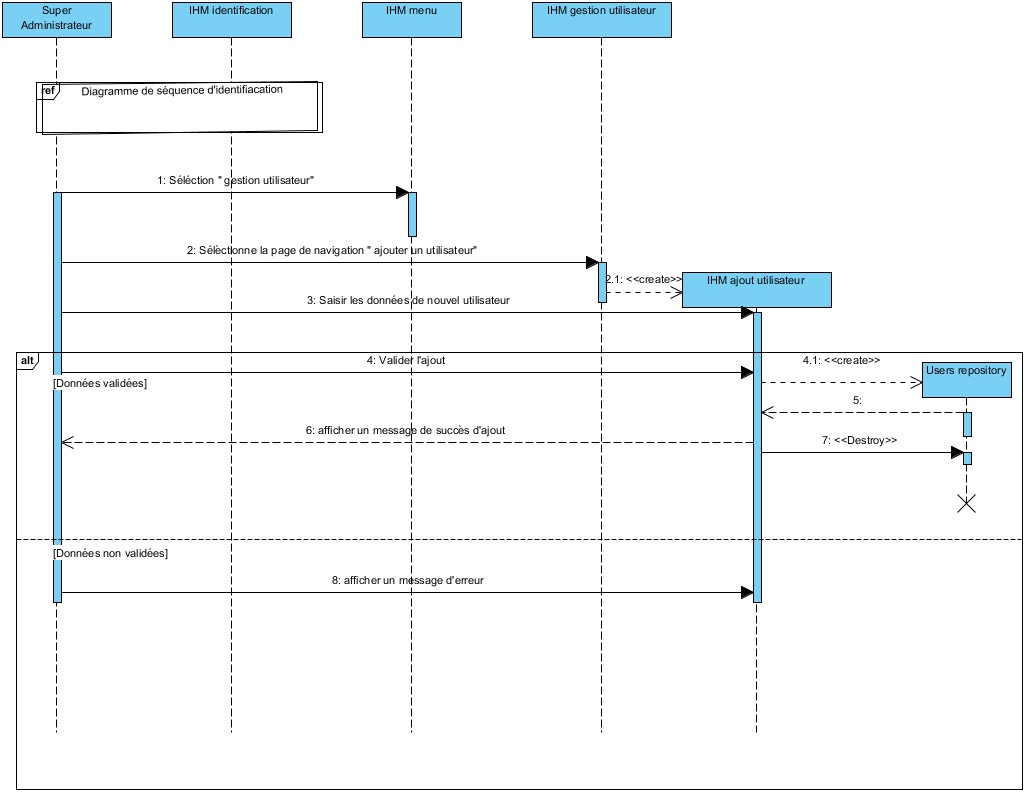
\includegraphics[height=4.7in]{DiagSeqAjouterUtilisateur.jpg}
\caption[Figure11 : Diagramme de séquence " gérer utilisateur "]{Diagramme de séquence " gérer utilisateur "}
\label{fig:pic11}
\end{figure}
\subsubsection{Diagramme de séquence "consulter la liste des utilisateurs"}
\begin{figure}[H]
\centering
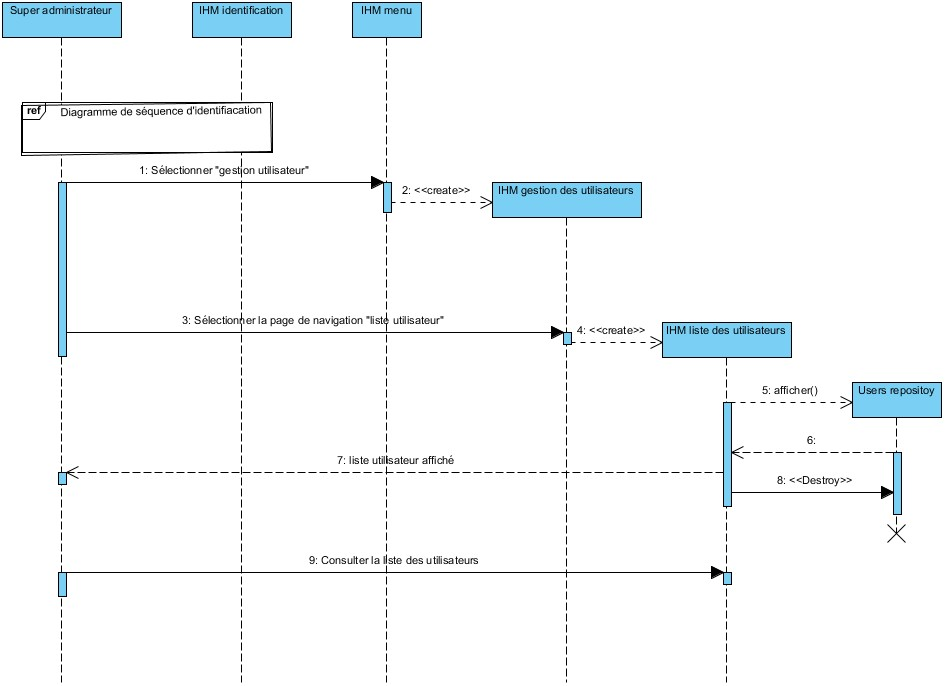
\includegraphics[height=4.7in]{DiagSeq2.jpg}
\caption[Figure12 : Diagramme de séquence " gérer liste des utilisateurs "]{Diagramme de séquence " gérer liste des utilisateurs "}
\label{fig:pic12}
\end{figure}

\subsection{Sprint 2 : Module d'assistance}
Au niveau du deuxième sprint de release, nous commençons par présenter le diagramme des classes nécéssaires à l'implémentation. Ensuite, on présentera
la conception avec les diagrammes de cas d'utilisation et de  séquences. 
\begin{enumerate}
\item[$\bullet$] \textbf{ Diagramme des classes}
\begin{figure}[H]
\centering
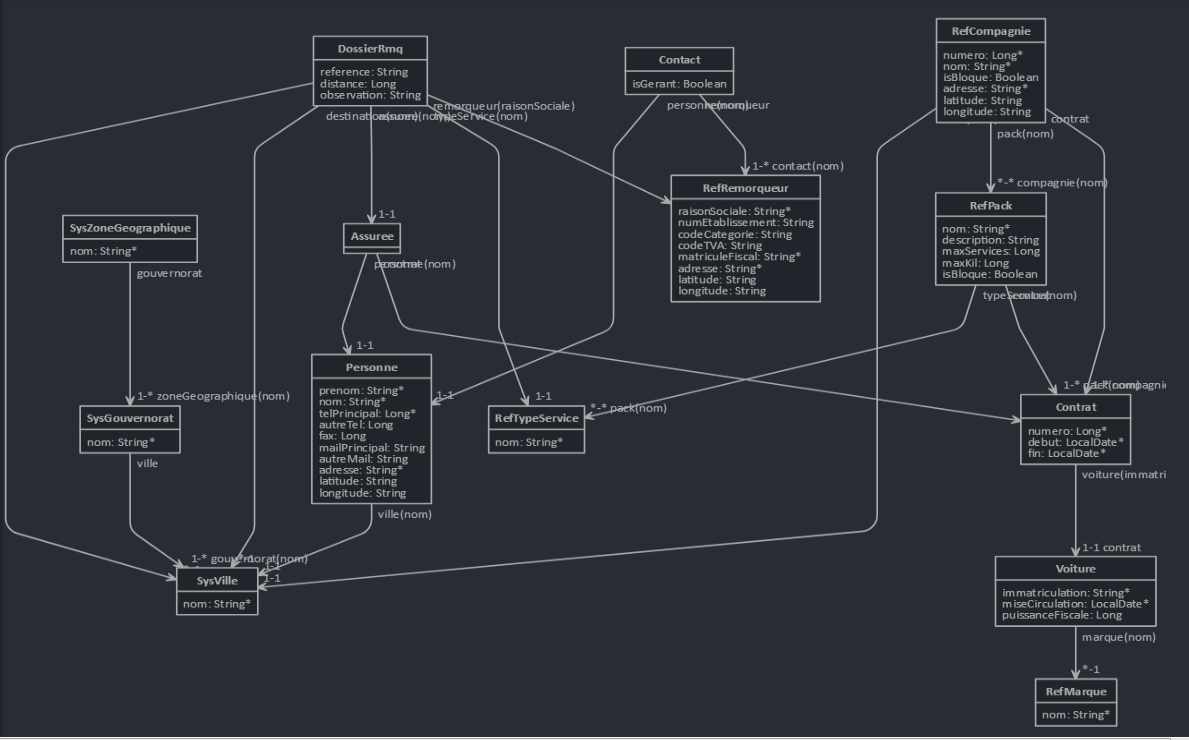
\includegraphics[height=4.8in]{DiagClasseModuleAssistance.PNG}
\caption[Figure13 : Diagramme de classe de module assistance]{Diagramme de classe de module assistance}
\label{fig:pic13}
\end{figure}
On va prendre l'exemple de gestion des remoqueurs.
\begin{figure}[H]
\centering
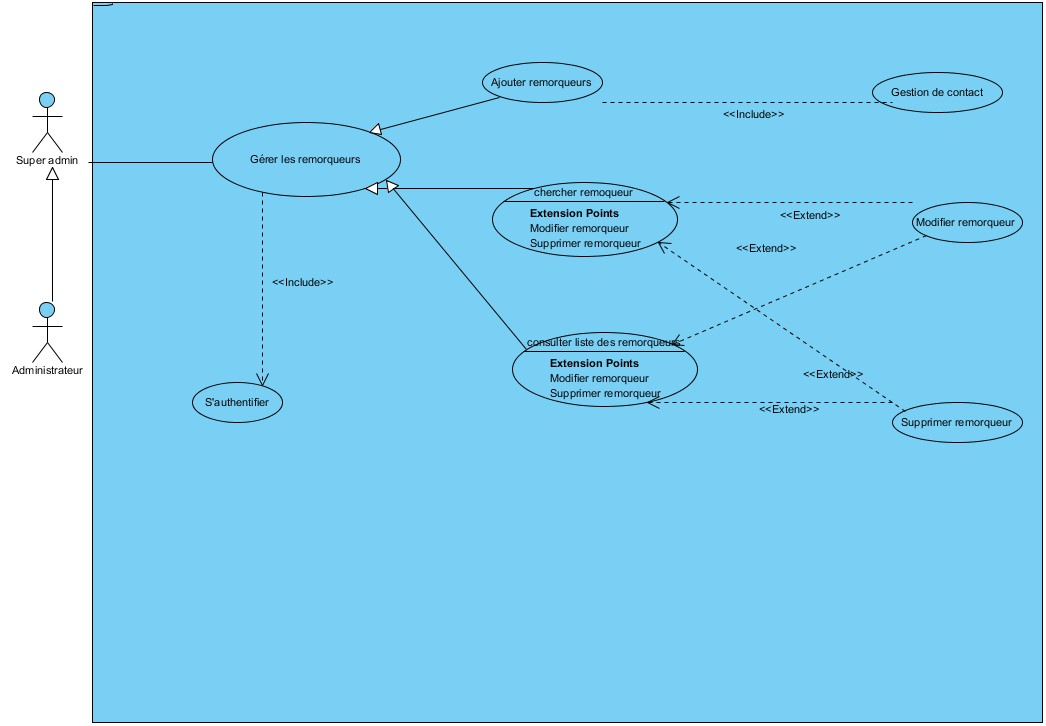
\includegraphics[height=4.8in]{UseCaseDiagram2.jpg}
\caption[Figure14 : Diagramme de cas d'utilisation " gérer remorqueurs "]{Diagramme de cas d'utilisation " gérer remorqueurs "}
\label{fig:pic14}
\end{figure}
Le diagramme de cas d'utilisation présenté par la figure \ref{fig:pic14} décrit la gestion des
remorqueurs par l'administrateur. Ce diagramme nous montre que l'administrateur ne peut faire sa gestion qu'après identification.Ainsi que la modification ou la suppression d'un remorqueur ne peut être effectuer qu'après consultation de liste des remorqueurs.
\end{enumerate}
\subsubsection{Description textuelle du cas d'utilisation "ajouter un remorqueur"}

Nous allons réaliser une description textuelle du scénario d'ajout d'un remorqueur
pour mieux connaître les étapes à suivre pour que l'administrateur réussit cette ajout.\\
Cette description est présentée par le tableau \ref{tab:tab8}
\begin{table}[H]
\centering
 \begin{tabularx}{\textwidth}{|X||X|}
\hline
 \textbf{Titre} & \textbf{ajouter un nouveau remorqueur} \\ \hline
\textbf{Résumé} & ajouter un nouveau remorqueur à la base de donnée \\
\hline
\textbf{Acteurs} &Super Administrateur et administrateur\\
\hline
\textbf{Précondition} & S'identifier \\
\hline
\textbf{Postcondition} & Un nouveau remorqueur est enregistré. \\
\hline
\textbf{Scénario nominal} & \begin{enumerate}
\item L'utilisateur saisie les données du nouveau remorqueur.
\item L'utilisateur appuie sur le bouton \guillemotleft sauvegarder \guillemotright pour valider l'ajout.
\item L'application affiche un message de succès.
\end{enumerate} \\
\hline
\textbf{Scénario alternatif} & \begin{enumerate}
\item L'utilisateur effectue une erreur de saisie.
\item L'application affiche un message d'erreur.
\item Le scénario nominal reprend au point 1.
\end{enumerate} \\
\hline
\end{tabularx}
\caption[tableau 8 : Tableau descriptif du cas d'utilisation "ajouter un remorqueur"]{Tableau descriptif du cas d'utilisation "ajouter un remorqueur"}
\label{tab:tab8}
\end{table}
\subsubsection{Diagramme de séquence "ajouter un remorqueur"}
\begin{figure}[H]
\centering
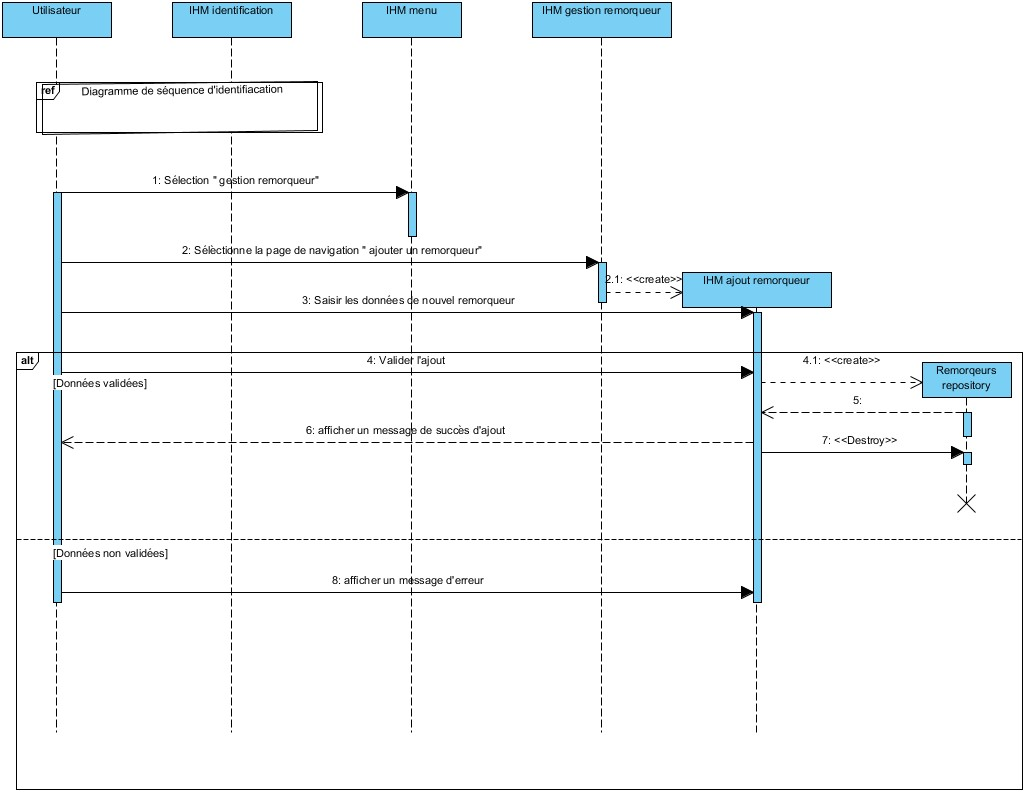
\includegraphics[height=5.4in]{DiagSeqAjouterRemorqueur.jpg}
\caption[Figure15 : Diagramme de séquence " gérer remorqueurs "]{Diagramme de séquence " gérer remorqueurs "}
\label{fig:pic15}
\end{figure}
\textbf{NB : } De même pour les autres classes.
\cleardoublepage
\subsection{Conclusion} 
A ce stade, nous avons réussi à développer les différentes tâches des modules d'administration et d'assistance. Dans le chapitre qui suit, notre effort sera consacré pour l'intégration des modules dans une seule application, le déploiment sur un serveur physique ainsi que la présention de quelques écrans pour la démonstration de
notre système.
\cleardoublepage
\setcounter{section}{3}
\setcounter{subsection}{0}
\section*{Chapitre 3 :  Release 2 " Déploiment de l'application et réalisation "}
\addcontentsline{toc}{section}{\numberline{} Chapitre 3 : Release 2 " Déploiment de l'application et réalisation "}
\subsection{Introduction}
Après avoir entamé le release de la gestion administration et gestion d'assistance,
nous pouvons maintenant passer au deuxième release \guillemotleft Déploiment et réalisation \guillemotright.
En effet, ce release constitue la dernière tâche  de notre projet puisqu'elle permet de mettre l'application en mode production et la societé peut ainsi profiter de ses fonctionnalités.
\subsection{Sprint 1 : Intégration des modules }
L'application se constitue par deux modules : \\
\begin{enumerate}
\item[$\bullet$] \textbf{ Administration}
\item[$\bullet$] \textbf{ Assistance }
\end{enumerate}
Le premier module consiste à gérer l'accès à l'application et gestion des rôles et d'utilisateur.
Il s'agit de deux rôles : Super administrateur et administrateur.\\
Le deuxième module contient pratiquement les fonctionnalités de l'application : gestion des contact, gestion des packs , gestion de dossier d'assuré et gestion des remorqueurs.\\
Les deux modules sont développés séparément sur des machines différentes et par des personnes différents. Dans ce sprint, l'objectif était d'assurer une bonne intégration sans conflit pour aboutir à une application fonctionnelle.
On a utlisé GIT, qui est un logiciel de gestion de versions.\\
On a aussi utilisé REDMINE qui est une application web libre de gestion de projets complète en mode web. 
\subsection{Sprint 2 : Réalisation }
\begin{titlepage}\centering
\vspace*{\fill}
\textbf{\LARGE ANNEXE }
\vspace*{\fill}
\end{titlepage}
\setcounter{page}{41}
\appendix
\subsubsection*{Pourquoi Scrum :}
\vspace{0.5cm}
\vspace{0.3cm}

\guillemotleft Scrum signifie mêlée au rugby. Scrum utilise les valeurs et l’esprit du rugby et les adapte aux projets de développement. Comme le pack lors d’un ballon porté au rugby, l’équipe chargée du développement travaille de façon collective, soudée vers un objectif précis. Comme un demi de mêlée, le Scrum Master aiguillonne les membres de l’équipe, les repositionne dans la bonne direction et donne le tempo pour assurer la réussite du projet. \guillemotright [1]\\\label{sec:hello}
Scrum est issu des travaux de deux des signataires du Manifeste Agile\footnote{Le manifeste agile est un texte rédigé et signé en 2001 par 17 experts dans le domaine de développement d’applications informatique.}, Ken Schwaber et Jeff Sutherland, au début des années 1990. Il appartient à la famille des méthodologies itératives et incrémentales et repose sur les principes et les valeurs agiles.\\
Le plus souvent, les experts de Scrum, même ses fondateurs, le décrivent comme un cadre ou un patron de processus orienté gestion de projet et qui peut incorporer différentes méthodes ou pratiques d’ingénierie.

S’il est difficile de définir la nature de Scrum, sa mise en place est beaucoup plus simple et peut être résumée par la Figure \ref{fig:pic8}. Le principe de base de Scrum est le suivant :
\begin{itemize}
\item[$\ast$] Dégager dans un premier lieu le maximum des fonctionnalités à réaliser pour former le backlog du produit,
\item[$\ast$] En second lieu définir les priorités des fonctionnalités et choisir lesquelles seront réalisé dans chaque itération,
\item[$\ast$]Par la suite focaliser l'équipe de façon itérative sur l’ensemble de fonctionnalités à réaliser, dans des itérations appelées Sprints,
\item[$\ast$]Un Sprint aboutit toujours sur la livraison d’un produit partiel fonctionnel appelé incrément.
\end{itemize}
\begin{figure}[H]
\centering
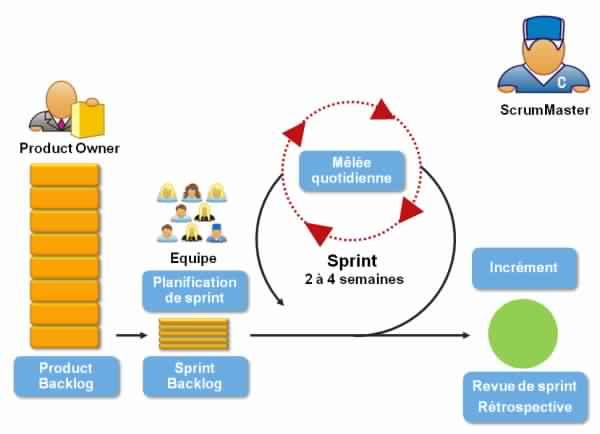
\includegraphics[height=2.5in]{methode-scrum.jpg}
\caption[Figure8 : Le processus Scrum]{Le processus Scrum[2]}
\label{fig:pic8}
\end{figure}
Le choix de Scrum comme une méthodologie de pilotage pour notre projet s’est basé sur les atouts de ce dernier. Il se résume comme suit:
\begin{itemize}
\item Plus de souplesse et de réactivité,
\item La grande capacité d’adaptation au changement grâce à des itérations courtes,
\item La chose la plus importante, c’est que Scrum rassemble les deux cotés théorique et pratique et se rapproche beaucoup de la réalité.
\end{itemize}
\subsection*{Equipe et rôles (Scrum) : }
\guillemotleft L’équipe a un rôle capital dans Scrum : elle est constituée dans le but d’optimiser la flexibilité et la productivité; pour cela, elle s’organise elle-même et doit avoir toutes les compétences nécessaires au développement du produit. Elle est investie avec le pouvoir et l’autorité pour faire ce qu’elle a à faire \guillemotright \footnote{C. Aubry, SCRUM le guide pratique de la méthode agile la plus populaire, Dunod, 2010.}\\
Bref, Scrum définit trois rôles qui sont : 

\textbf{Le Product Owner (le propriétaire du produit)} : c’est une personne qui porte la vision du produit à réaliser, généralement c’est un expert dans le domaine.\\
\label{sec:hello1}
\textbf{Le Scrum Master (le directeur de produit) } : c'est la personne qui doit assurer le bon déroulement des différents sprints du release, et qui doit impérativement maitriser Scrum. \\

\textbf{Le Scrum Team (l’équipe de Scrum)} : constitué des personnes qui seront chargées d’implémenter les différents besoins du client. Bien évidemment, cette équipe sera constituée des développeurs, des testeurs, etc.\\
Dans le contexte de notre projet, M. Aouadi Bessem sera le directeur de produit, et M. Toukebri Mohamed Arbi sera le propriétaire et moi Choubani Amir  je forme le membre de l’équipe Scrum.
\subsection*{Backlog de produit : }
\textbf{Rang} : Pour les user stories ayant la même priorité, un rang est assigné pour indiquer l'ordre dans lequel l'équipe doit les implémenter.\\
\textbf{Estimation} : Sert à estimer l’effort nécessaire à une équipe pour implémenter une fonctionnalité. Elle prend en compte l’effort pour le développement.\\
\textbf{Importance} : C’est un nombre qu'attribue le product owner à l'histoire : plus l'importance est grande, plus l'histoire devra être traitée en priorité.\\
\textbf{Priorité} : Le product Owner classe les user story par ordre de priorité dans le Backlog produit en travaillant avec le client pour savoir ce qui est important pour lui.\\
On utilise la suite de fibonacci pour attribuer les priorités.\\ 
\textbf{Description} : Elle permet de décrire les user stories. Généralement, pour rendre ce nom explicite, une bonne façon de procéder est d'utiliser le Template suivant :  \guillemotleft En tant que X, je veuxY, afin de... \guillemotright. \\
\label{sec:hello2}
\subsection*{Spring Boot : }
 Le framework propose une approche dogmatique de la configuration, qui permet d'éviter aux développeurs de redéfinir la même configuration à plusieurs endroits du code. Dans ce sens, Boot se veut d'être un acteur majeur dans le secteur croissant du développement d'applications rapide.\\
Spring Boot facilite la création d'applications et de services de production, avec un minimum d'encombrement absolu. Il prend une vue d'opinion de la plate-forme Spring afin que les utilisateurs nouveaux et existants puissent rapidement accéder aux bits dont ils ont besoin.
\label{sec:hello3}
\subsection*{Architecture MVC : }
La partie Modèle d’une architecture MVC encapsule la logique métier ainsi que l’accès aux données. Il peut s’agir d’un ensemble de fonctions ou de classes.Ceci est géré par Spring Boot.\\
La partie Contrôleur gère la dynamique de l’application. La partie Vue s’occupe des interactions avec l’utilisateur : présentation, saisie et validation des données.Ceci est géré par Angular.
 Elle fait le lien entre l’utilisateur et le reste de l’application.
La demande de l’utilisateur est reçue et interprétée par le Contrôleur. Celui-ci utilise les services du Modèle afin de préparer les données à afficher. Ensuite, le Contrôleur fournit ces données à la Vue, qui les présente à l’utilisateur sous la forme d’une page HTML.
\label{sec:hello4}
\cleardoublepage
\bibliographystyle{unsrt}
\begin{thebibliography}{1}
\bibitem{1} \textcolor{blue}{\url{https://developers.google.com/places/javascript/?hl=fr}} consulté le 12/08/17
\bibitem{2} \textcolor{blue}{\url{ http://ineumann.developpez.com/tutoriels/alm/agile_scrum/ }} consulté le 12/08/17
\bibitem{3} \textcolor{blue}{\url{http://www.redcad.org/members/tarak.chaari/cours/coursUML.pdf }} consulté le 13/08/17
\bibitem{4} \textcolor{blue}{\url{http://www.redcad.org/members/tarak.chaari/cours/coursUML.pdf }} consulté le 13/08/17
\bibitem{5} \textcolor{blue}{\url{https://blog.netapsys.fr/wp-content/uploads/2017/03/ }} consulté le 13/08/17
\bibitem{6} \textcolor{blue}{\url{http://blog.oxiane.com/wp-content/uploads/2016/02/ }} consulté le 13/08/17
\bibitem{7} \textcolor{blue}{\url{http://blog.viseo-bt.com/wp-content/uploads/2012/03/}} consulté le 13/08/17
\bibitem{8} \textcolor{blue}{\url{http://telecharger.cnet.com/Visual-Paradigm-for-UML/}} consulté le 13/08/17
\end{thebibliography}

\end{document}